\chapter{Запрос и управление XML-данными}
\section{Возвращение результатов в виде XML
с помощью предложения FOR XML}


\begin{lstlisting}[label=lst:funcReturn, language=sql]
	WITH XMLNAMESPACES('TK461-CustomersOrders' AS co) S
	ELECT [co:Customer].custid AS [co:custid],
	 [co:Customer].companyname AS [co:companyname],
	 [co:Order].orderid AS [co:orderid],
	 [co:Order].orderdate AS [co:orderdate]
	FROM Sales.Customers AS [co:Customer]
	 INNER JOIN Sales.Orders AS [co:Order]
	 ON [co:Customer].custid = [co:Order].custid
	WHERE [co:Customer].custid <= 2
	 AND [co:Order].orderid %2 = 0
	ORDER BY [co:Customer].custid, [co:Order].orderid
	FOR XML AUTO, ELEMENTS, ROOT('CustomersOrders'); 
\end{lstlisting}


\begin{figure}[h!]
	\begin{center}
		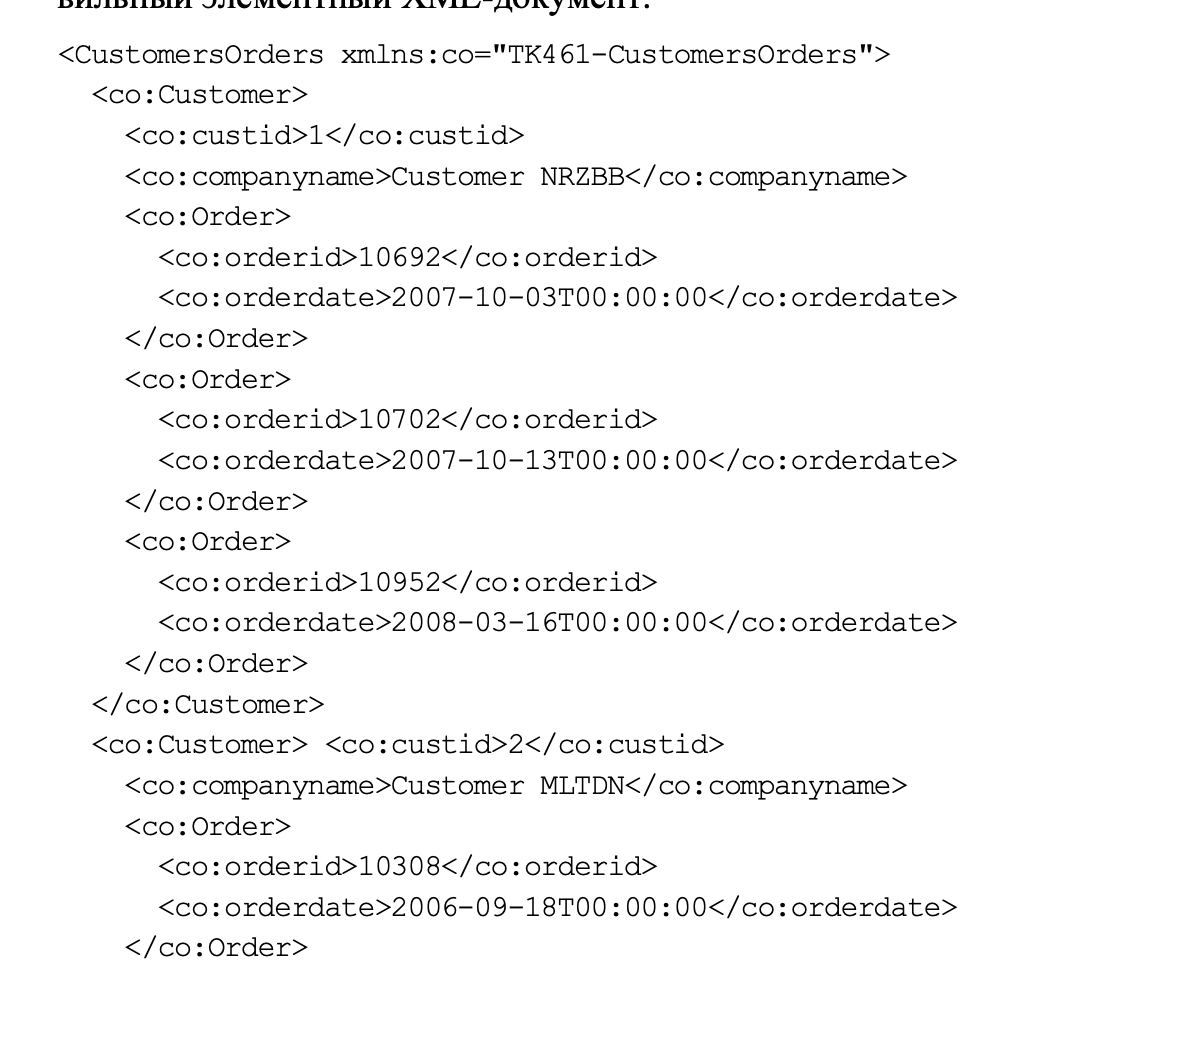
\includegraphics[width=0.8\textwidth]{img/res16.png}
	\end{center}
	\captionsetup{justification=centering}
\end{figure}


\subsection{Режим FOR XML PATH}
С помощью двух последних возможностей предложения FOR XML — параметров
EXPLICIT и PATH — можно вручную определять возвращаемый XML. Используя
эти два параметра, вы получаете полный контроль над возвращаемым XMLдокументом.


\begin{lstlisting}[label=lst:funcReturn, language=sql]
	SELECT Customer.custid AS [@custid],
	Customer.companyname AS [companyname]
   FROM Sales.Customers AS Customer
   WHERE Customer.custid <= 2
   ORDER BY Customer.custid
   FOR XML PATH ('Customer'), ROOT('Customers'); 
\end{lstlisting}

\begin{figure}[h!]
	\begin{center}
		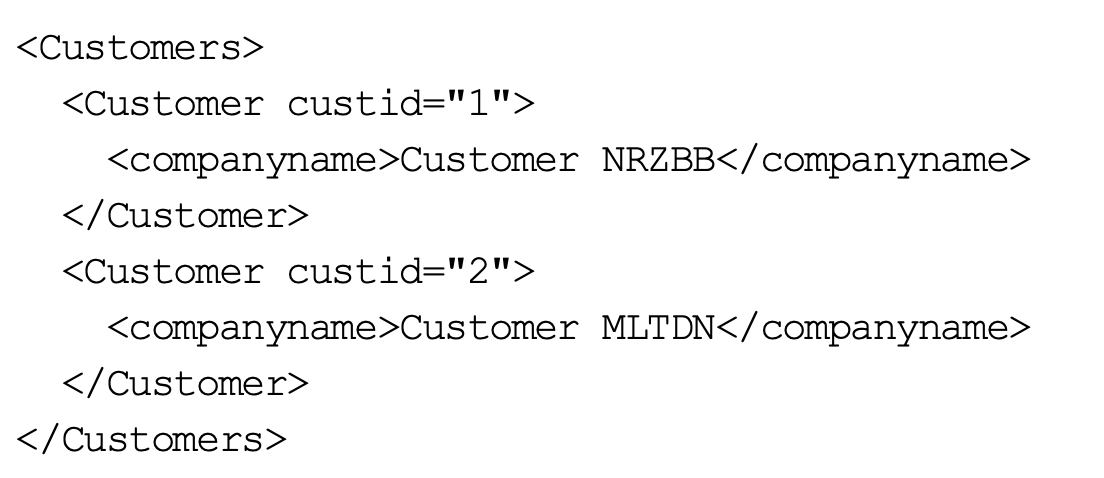
\includegraphics[width=0.8\textwidth]{img/xml.png}
	\end{center}
	\captionsetup{justification=centering}
\end{figure}


\section{Запрос XML-данных с помощью XQuery}

\begin{lstlisting}[label=lst:funcReturn, language=sql]
	DECLARE @x AS XML;
	SET @x=N'
	<root>
	 <a>1<c>3</c><d>4</d></a>
	 <b>2</b>
	</root>';
	SELECT
	 @x.query('*') AS Complete_Sequence,
	 @x.query('data(*)') AS Complete_Data,
	 @x.query('data(root/a/c)') AS Element_c_Data; 
\end{lstlisting}

\begin{figure}[h!]
	\begin{center}
		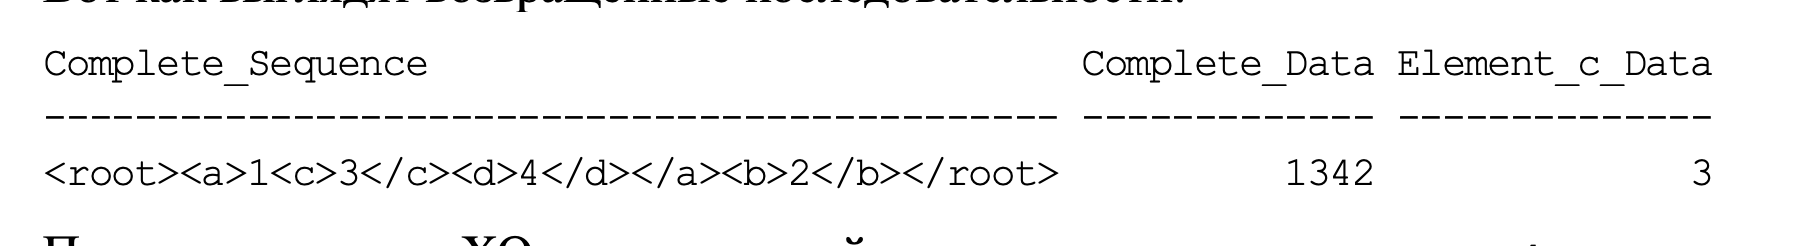
\includegraphics[width=0.8\textwidth]{img/xquery.png}
	\end{center}
	\captionsetup{justification=centering}
\end{figure}

Первое выражение XQuery — простейшее возможное выражение path, которое выбирает все из экземпляра XML; второе использует функцию data() для извлечения
атомарных значений данных из всего документа; третье использует функцию
data() для извлечения атомарных значений данных только из элемента. 


\subsection*{Резюме занятия}
\begin{itemize}
	\item Язык XQuery можно использовать в запросах T-SQL, чтобы запрашивать XMLданные. 
	\item Язык XQuery поддерживает собственные типы данных и функции. 
	\item Выражение XPath используется для навигации по экземпляру XML. 
	\item Настоящая сила XPath заключена в выражениях FLWOR. 
\end{itemize}